\subsection{Sensing Subsystem Testing}
\label{sec:sensing_subsystem_testing}

\subsubsection{Component Testing}
Three components in the Sensing subsystem required testing on arrival.
\begin{itemize}
    \item The Optical Sensors
    \item The Linear Actuator
    \item The Transimpedance Amplifier Board
\end{itemize}

\paragraph{} A small transimpedance amplifier was constructed on a breadboard in the electrical lab to convert nA of electrical current to mV of electrical voltage. With an oscilloscope, the photodetectors were determined to be measuring optical power, with varying ambient light levels and light sources increasing the voltage within a measurable range.

\paragraph{} Similarly, the stepper motor was connected to a Texas Instruments evaluation board with motor controller software. The stepper motor turned the screw, successfully carrying the mount in steps along the stroke length of the rail.

\paragraph{} When the circuit board arrived it was installed with insulating spacers onto the metal mount on the linear rail and both components were optically isolated inside an opaque box. A fiber and diffraction grating were aligned inside to allow outside light to be dispersed in front of the rail. The photodetectors were successfully amplified by the circuit board, prompting the team to move on to permanent installation of each of the optical components.

\subsubsection{Performance Testing}

In order to evaluate the performance of the system, two tests were conducted.

\paragraph{} The first test was an integration test to connect all parts of the Spectrometer subsystem and generate a spectrograph. For the purposes of this test, it did not matter what data was produced, only that the system was capable of recording data. The light collection cone was set on top of a large piece of flattened aluminum foil. See the two resulting datasets below.

\begin{figure}[H]
    \caption{Aluminum Test VIS Data}
    \centering
    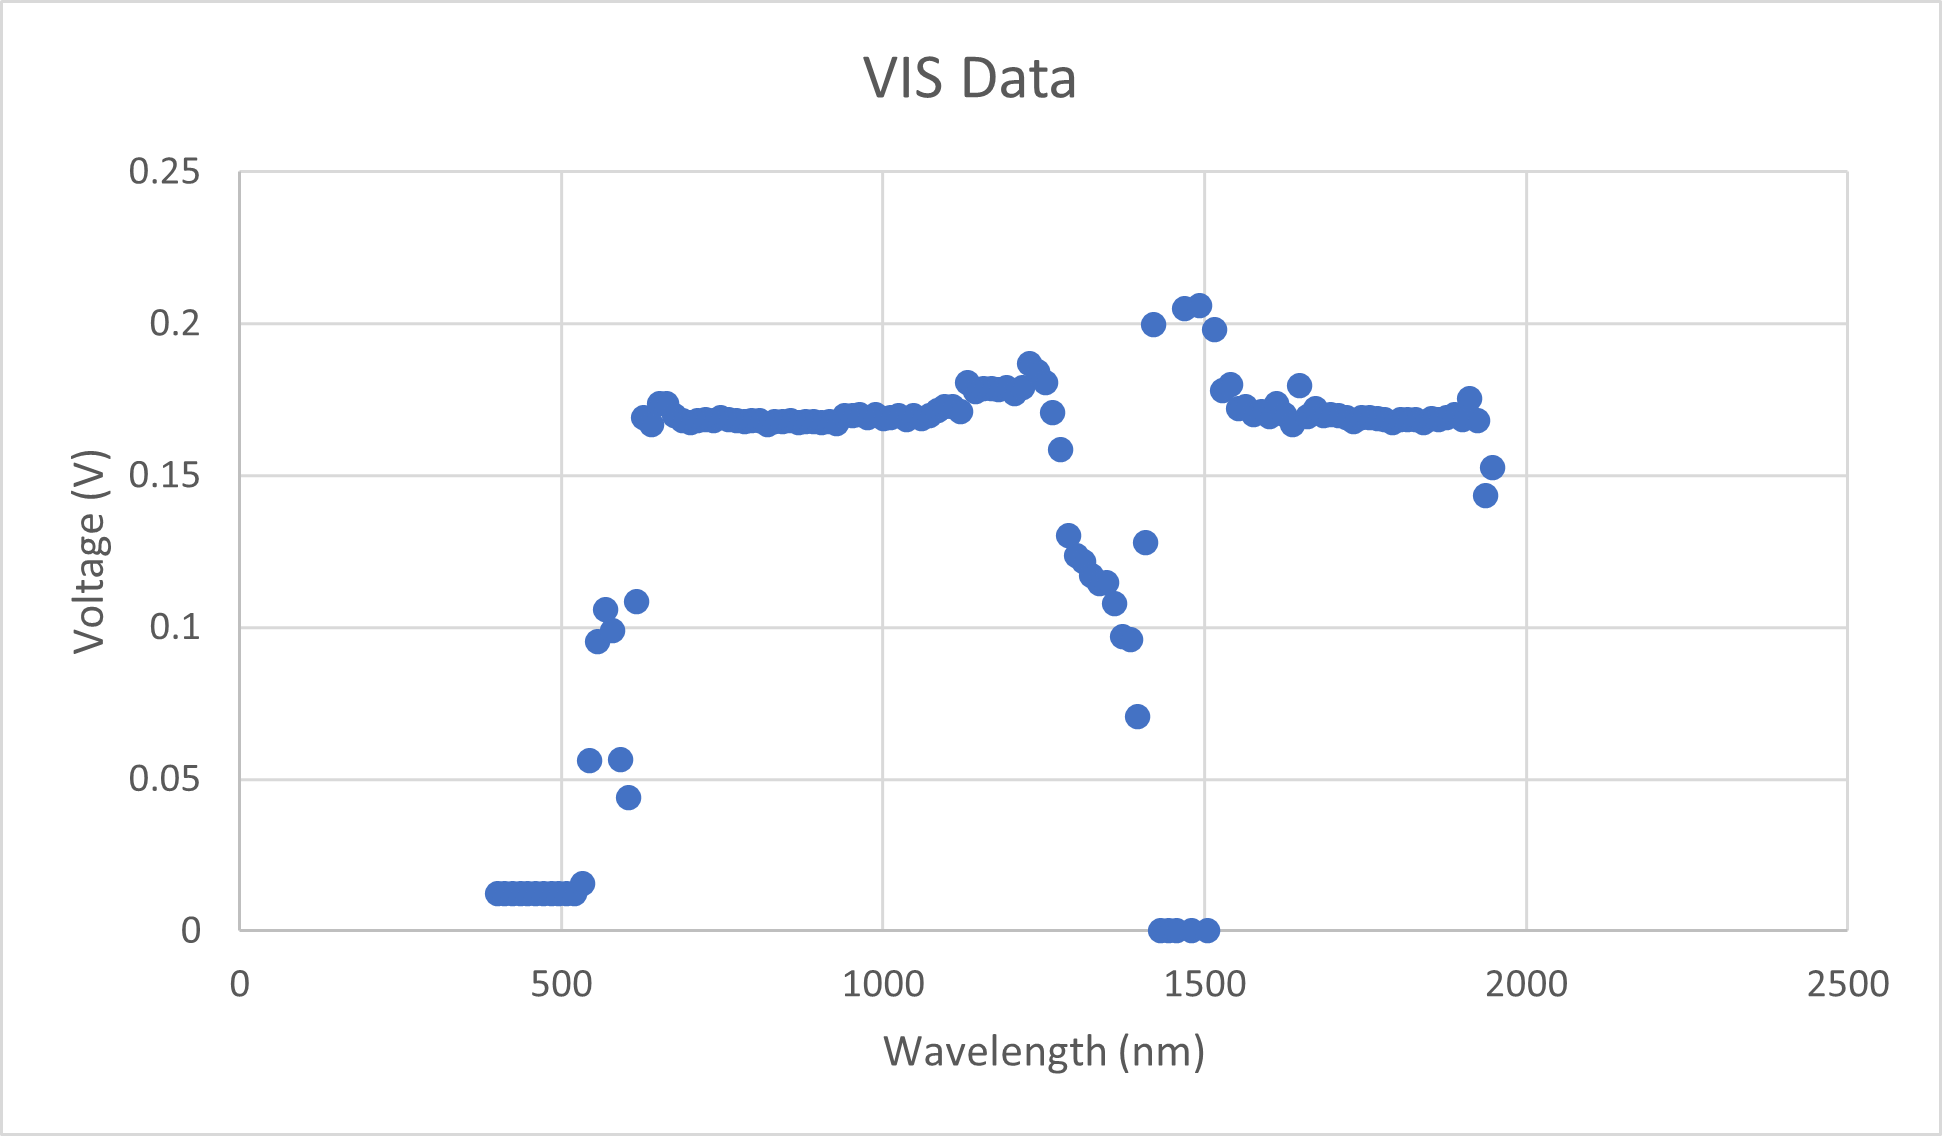
\includegraphics[scale=1]{images/Aluminum VIS Data.png}
\end{figure}

\begin{figure}[H]
    \caption{Aluminum Test NIR Data}
    \centering
    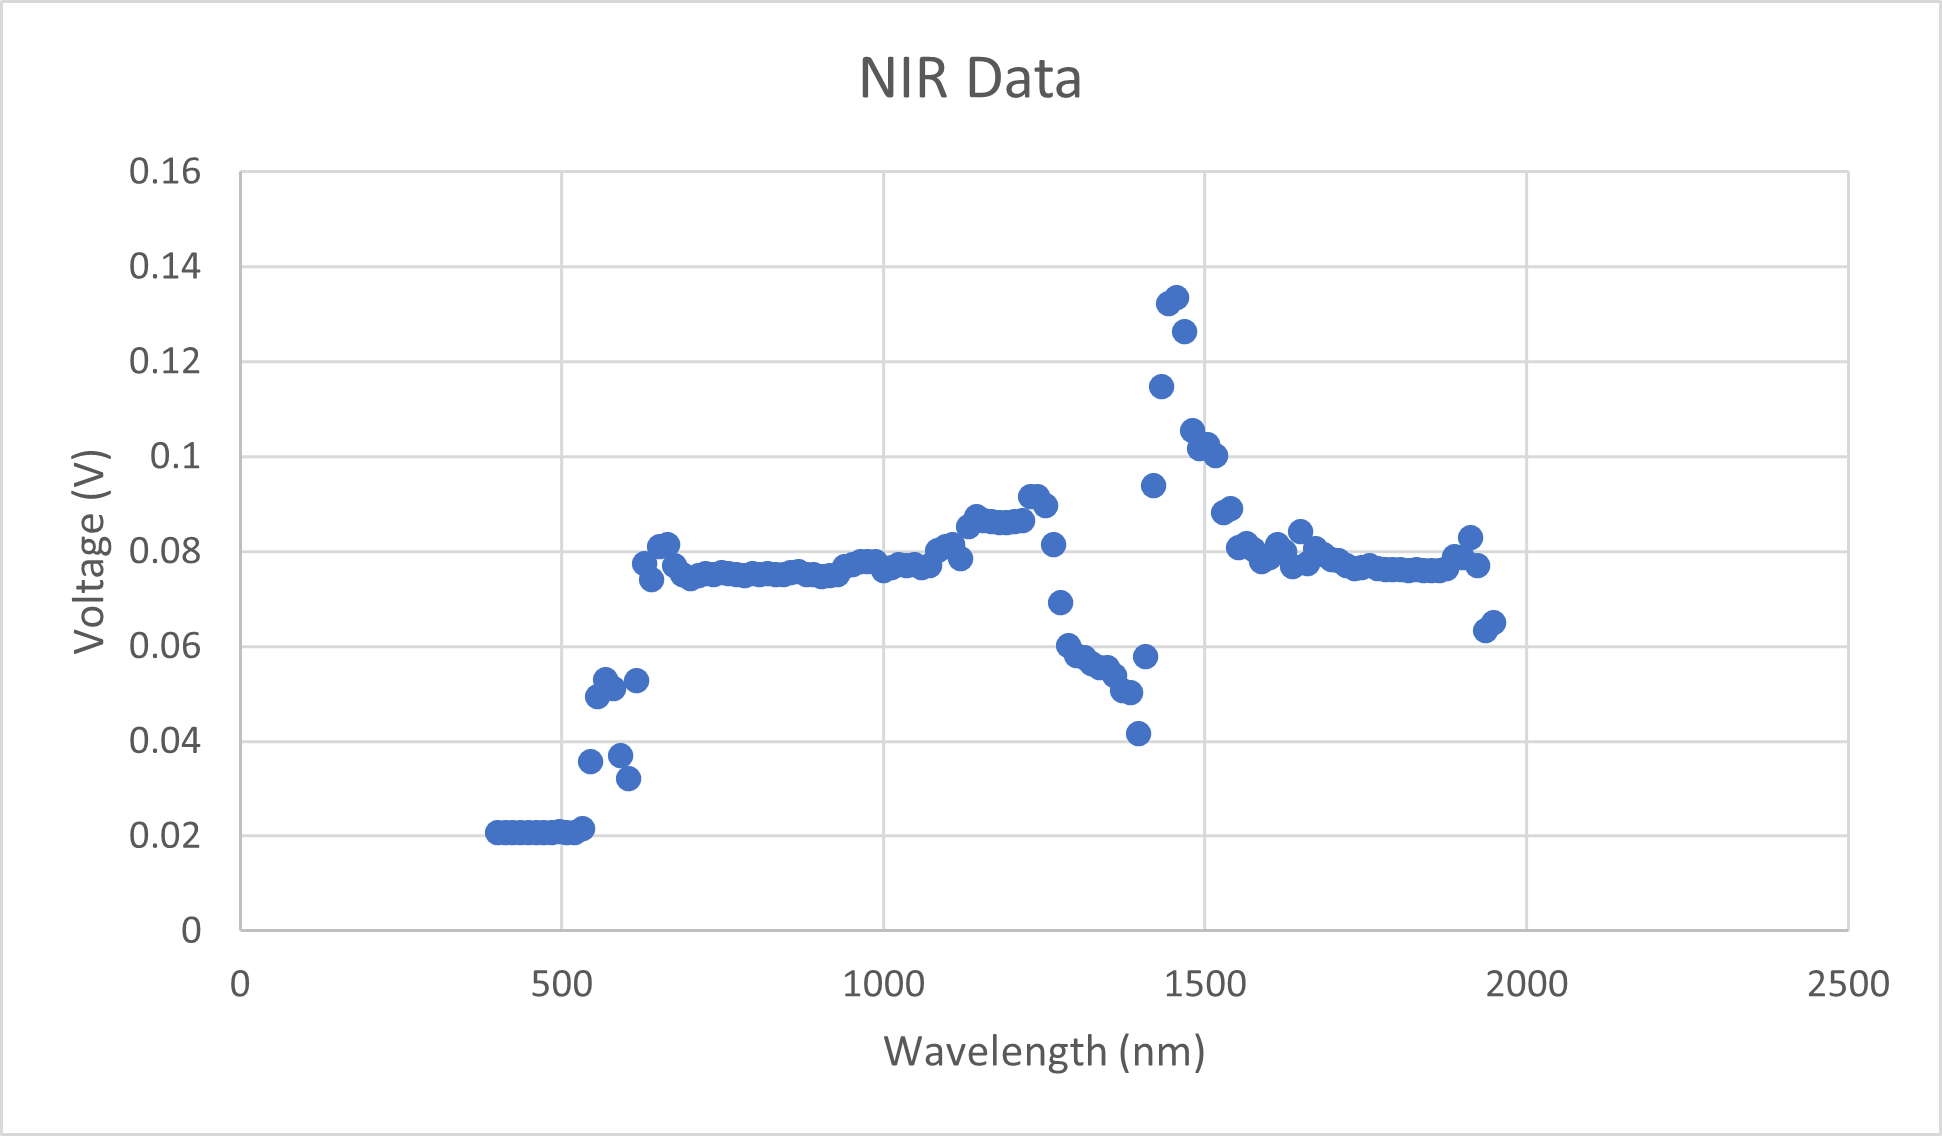
\includegraphics[scale=1]{images/Aluminum NIR Data.png}
\end{figure}

\paragraph{} The Second Test was to take three different soil samples and determine whether the spectrometer data was significant. To conduct this test, two fertilized bags of soil were purchased from a hardware store and one sample was collected from the ground nearby. The results of these tests are below as well.

\begin{figure}[H]
    \caption{Miracle Grow Potting Mix Soil with 0.21 0.11 0.16 fertilizer}
    \centering
    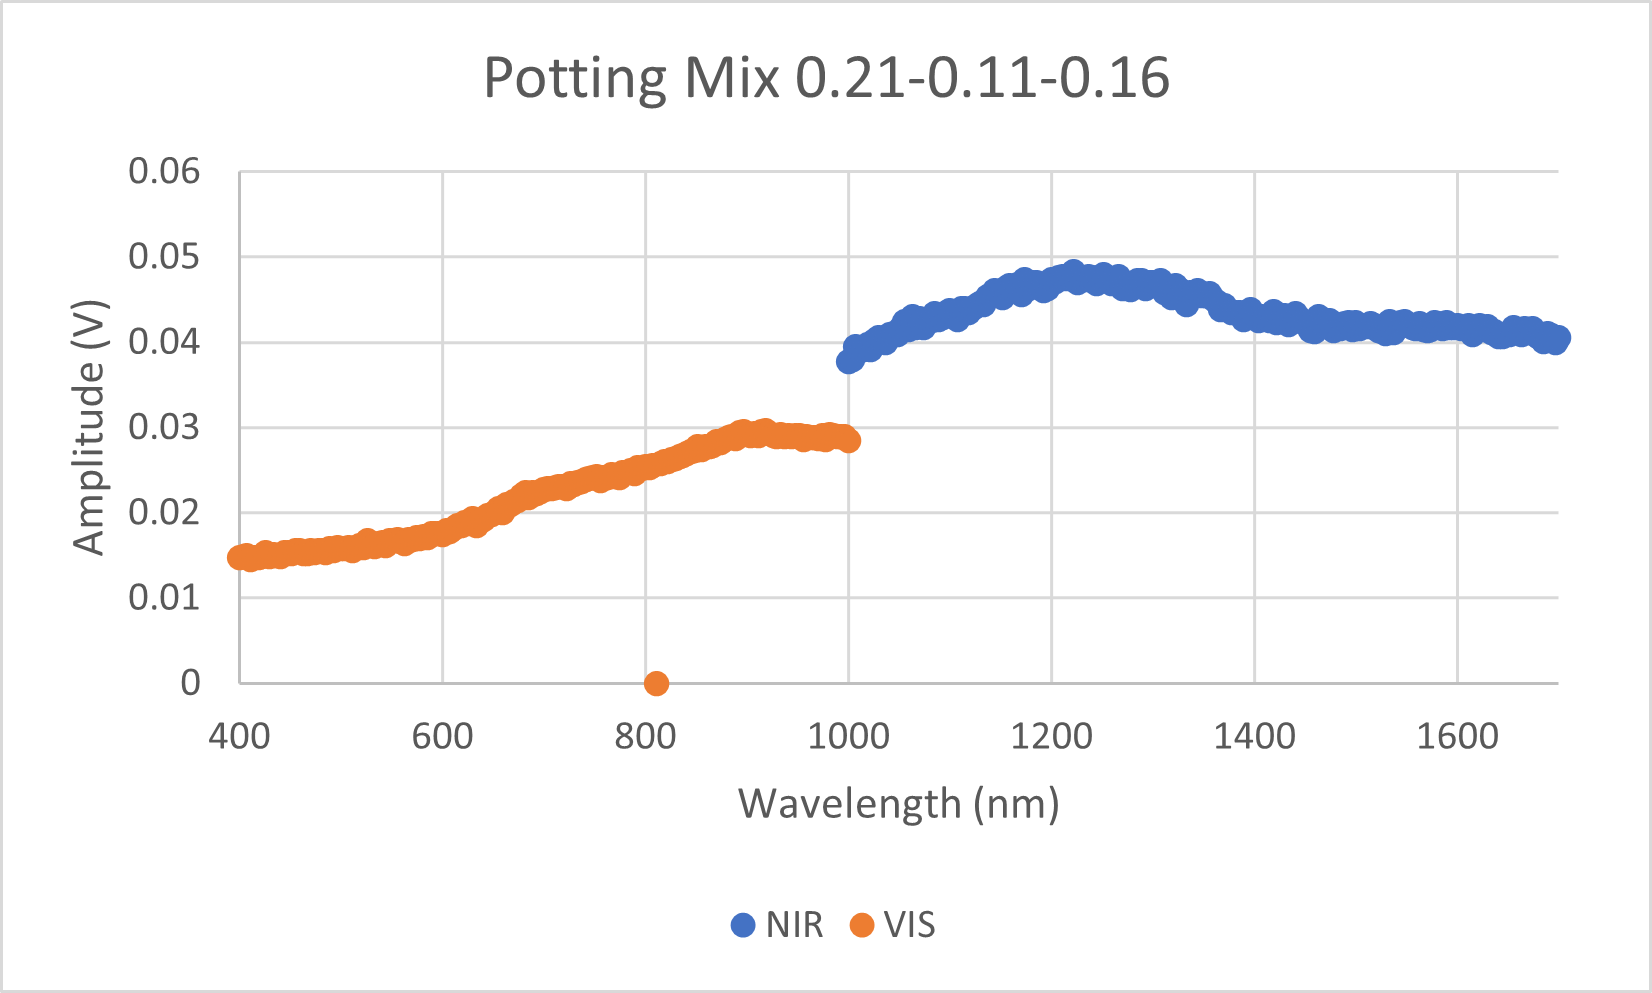
\includegraphics[scale=0.5]{images/Data1.png}
\end{figure}

\begin{figure}[H]
    \caption{Miracle Grow Performance Composted Manure with 0.19 0.03 0.03 fertilizer}
    \centering
    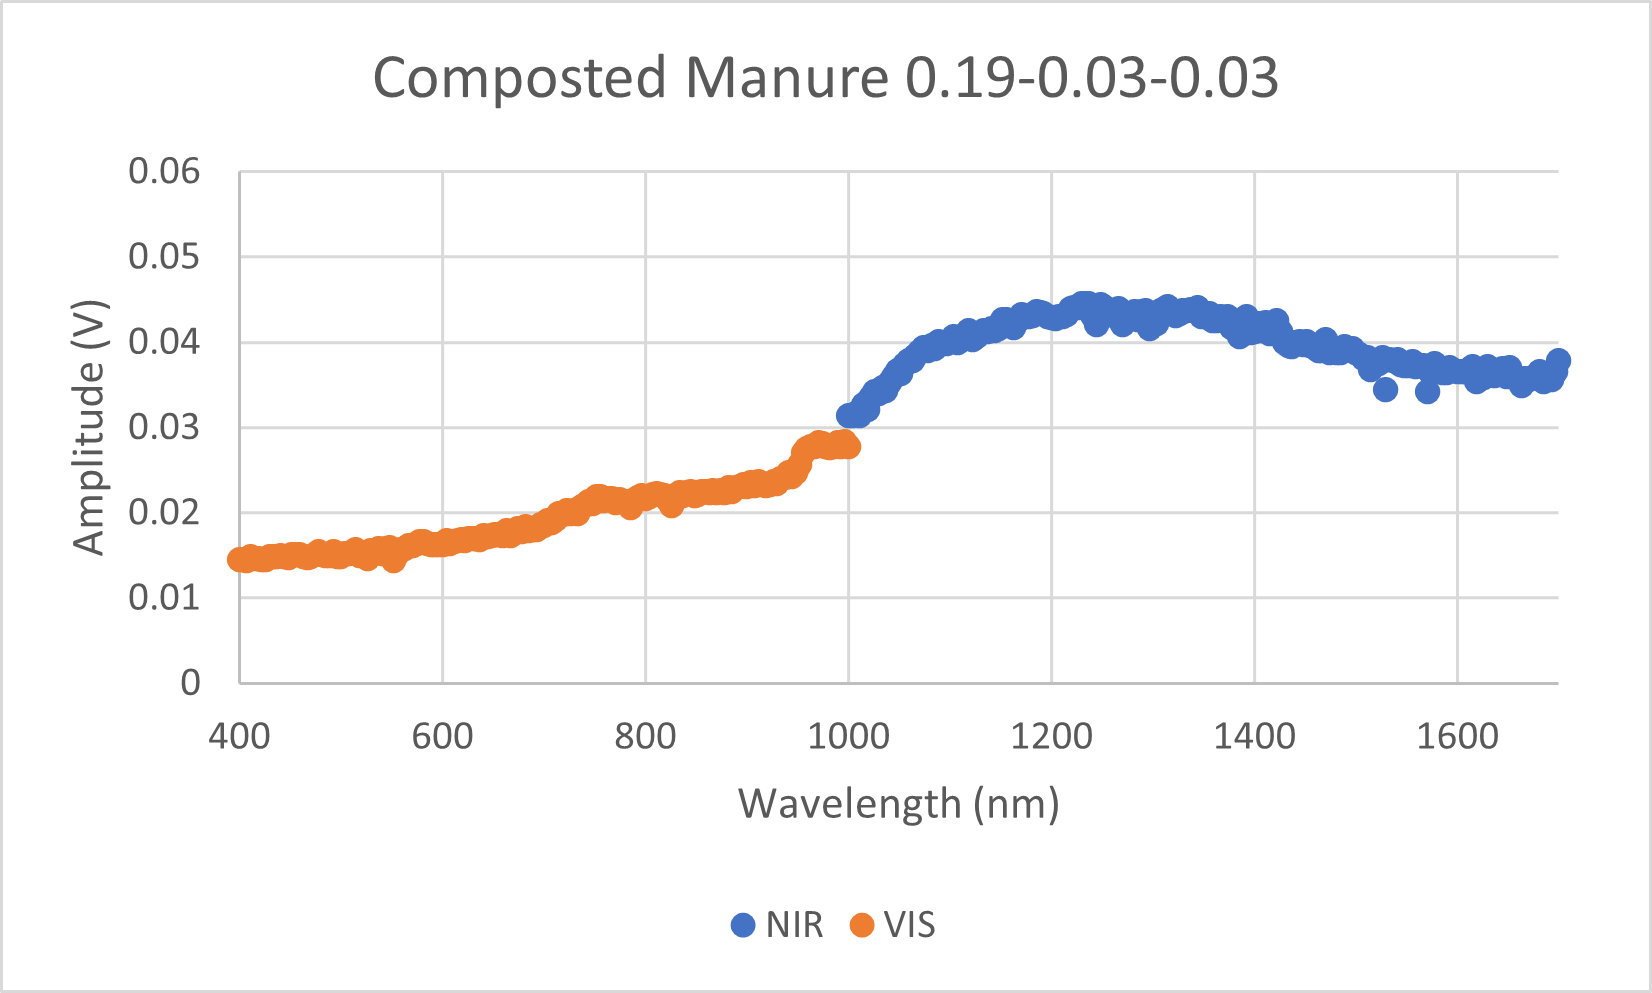
\includegraphics[scale=0.5]{images/Data2.png}
\end{figure}

\begin{figure}[H]
    \caption{Sandy Soil from University Grounds}
    \centering
    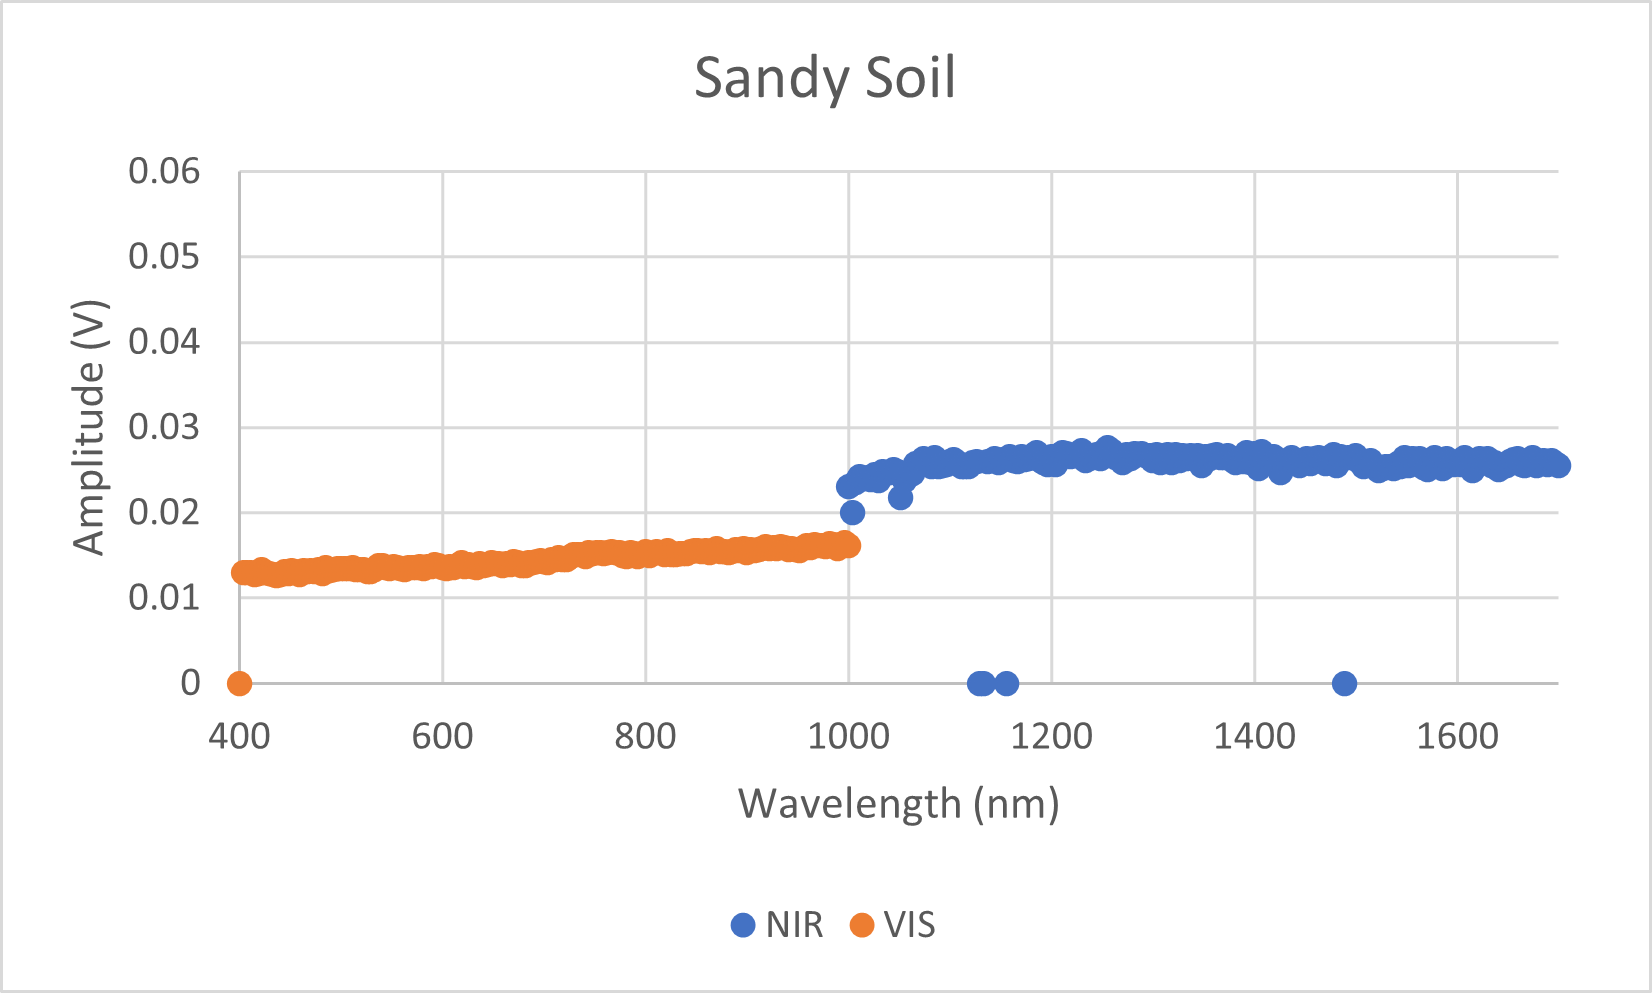
\includegraphics[scale=0.5]{images/Data3.png}
\end{figure}

These tests proved successful. At this time there is a call to cease activity on the project, and further tests will not be conducted. However, if there were more time to develop the system, the next test would be to engage the full resolution of the device in measurement and begin calibrating it against larger and larger datasets. 
